% Condensed edition, September 2026. Source tables and figures are generated by main.R.
% Compile from paper/: pdflatex concise_20_pages; bibtex concise_20_pages;
% pdflatex concise_20_pages; pdflatex concise_20_pages.
\documentclass[12pt,a4paper]{article}
\usepackage[T1]{fontenc}
\usepackage[utf8]{inputenc}
\usepackage{lmodern,amsmath,booktabs,threeparttable,graphicx,geometry,setspace}
\geometry{margin=2.45cm}
\setstretch{1.38}
\setlength{\parskip}{0pt}
\renewcommand{\topfraction}{0.9}
\renewcommand{\bottomfraction}{0.8}
\renewcommand{\textfraction}{0.06}
\renewcommand{\floatpagefraction}{0.68}
\setcounter{topnumber}{3}\setcounter{totalnumber}{4}
\usepackage[authoryear,round]{natbib}
\usepackage[colorlinks=true,linkcolor=blue,citecolor=blue,urlcolor=blue]{hyperref}
\newcommand{\sym}[1]{\ensuremath{^{#1}}}
\newcommand{\Mother}{\text{Mother}}
\newcommand{\Post}{\text{Post}}
\newcommand{\WFH}{\text{WFH exposure}}
% Generated by scripts/export_paper_tables.R from a pipeline run. Do not edit by hand.
\newcommand{\autonoteHours}{No coefficient is dropped for collinearity in any column.}
\newcommand{\autonoteSubgroup}{The Arab-women DiD drops the religion category `other', constant on that sample; the Arab-women DDD drops the religion category `other', constant on that sample; no other column drops a coefficient.}
\newcommand{\autonoteChildAge}{No coefficient is dropped for collinearity in any column.}
\newcommand{\autonoteExtensive}{No coefficient is dropped for collinearity in any column.}

\title{Did Remote Work Narrow the Motherhood Penalty?\\
\large Evidence on Weekly Hours from Israel, 2017--2023}
\author{Inbal Moryles \and Nitzan Zacharia\\
\small Tel Aviv University, The Eitan Berglas School of Economics}
\date{September 2026}
\begin{document}
\maketitle
\begin{abstract}
We study whether the expansion of work from home (WFH) changed employed mothers' usual weekly hours in Israel. Using Labor Force Survey observations from 2017--2019 and 2021--2023, we compare mothers with other women across occupations that differ in their capacity for remote work. The average difference-in-differences estimate is 0.23 hours (SE 0.18). The triple interaction with an Israeli-calibrated occupational exposure score is 3.22 hours per unit (SE 1.02), equivalent to 0.64 hours per standard deviation of exposure. The estimated top-to-bottom quartile contrast is 1.71 hours; an unrestricted quartile model suggests that the response is concentrated in the highest-exposure occupations. Permutation and wild-bootstrap tests give $p=0.032$ and $p=0.056$, respectively. These associations are consistent with flexibility easing some mothers' time constraints, subject to the design's exposure-measurement and parallel-trend assumptions. The employment interaction is too imprecise for a comparable conclusion.
\end{abstract}

\section{Introduction}\label{sec:intro}
The expansion of remote work offers a way to study a long-standing labor-market question: whether greater flexibility reduces the work constraints associated with motherhood. \citet{harrington2025} find increases in US mothers' employment and income relative to other women's in occupations with greater access to WFH. We ask how the corresponding change appears in Israeli women's \emph{usual weekly hours}, conditional on working. Hours are a distinct margin: an employed mother may increase paid work without changing employment status, while an increase in income could also reflect pay rather than hours.

The comparison matters in Israel, where fertility is relatively high among OECD countries \citep{oecd2025fertility}. Remote work can save commuting time and permit scheduling around care, but the released time need not be devoted to paid work. It could instead be allocated to domestic work or leisure. Firms may also reorganize jobs in ways that alter hours independently of individual flexibility. The sign and distribution of an hours response are therefore empirical questions.

We combine three contrasts in Israeli Central Bureau of Statistics (CBS) Labor Force Survey data: mothers versus women with no child younger than 17 in their household; 2017--2019 versus 2021--2023; and occupations with greater versus lesser WFH exposure. The third contrast uses an occupational task score that is partly adjusted to Israeli practice. Its identifying assumption concerns how the \emph{motherhood gap within occupations} would otherwise have evolved across different exposure levels. We examine this assumption with pre-period event studies and assess the exposure score, sorting, sample selection, outcome coding and inference in separate checks.

The average change in the hours gap is small: the difference-in-differences (DiD) estimate is 0.228 hours (SE 0.181). The exposure interaction is 3.224 hours per unit of the calibrated score (SE 1.022), or 0.640 hours per standard deviation. At the mean scores of the highest and lowest exposure quartiles, the fitted difference is 1.71 hours per week. An alternative specification with separate quartile effects puts the contrast at 1.844 hours (SE 0.595), with little evidence of a smooth response through the first three quartiles. The positive pattern is most pronounced among mothers of young children. An analogous regression for fathers has a negative, less precise exposure gradient. These results describe differences associated with access to remote-capable work; they do not isolate a randomized effect of WFH itself.

The paper first places the question in the literature, then explains the sample and exposure measure. Descriptive patterns precede the empirical strategy and results. The discussion interprets the conditional-hours finding, and the limitations specify what the design cannot establish. The employment outcome is included as a secondary analysis because its exposure interaction is not estimated precisely enough to resolve an effect of the size found in related US work.

\section{Literature Review}\label{sec:lit}
Research on the child penalty documents persistent losses in mothers' earnings that reflect both reduced hours and changes in employment and job choice \citep{kleven2019denmark,kleven2019countries}. \citet{goldin2014} connects gender pay differences to the high reward for long, uninterrupted hours in some jobs. WFH could ease a constraint on hours if it reduces travel and makes schedules more adaptable. Workers' willingness to accept lower pay for a remote-work option shows that such flexibility has value \citep{maspallais2017}; evidence on the return to long hours also suggests that the gains may vary across occupations \citep{cortespan2019}. For Israel, \citet{buzaglo2023} emphasize sorting within firms, which an occupation-level exposure measure cannot fully capture.

Evidence on how remote work changes hours is mixed. Time-diary work finds that remote days can shift time toward both paid work and care \citep{pabilonia2022}, while a study of information-technology workers finds longer working time without a comparable increase in output \citep{gibbs2023}. Experimental studies identify changes in work arrangements and household allocation \citep{bloom2015,angelici2024}. Lockdown-era evidence instead reflects simultaneous school and workplace disruptions \citep{alon2020,adamsprassl2020,yaish2021}; our later period is informative about a different setting, although 2021 still includes restrictions. Selection into WFH can differ from the effect of working remotely \citep{emanuelharrington2024}. For that reason, the analysis is organized around the capacity of an occupation to accommodate remote work rather than a worker's reported WFH status.

Our closest comparator is \citet{harrington2025}, whose outcomes are US employment and income. We focus on Israeli hours, an outcome more directly tied to the time-constraint mechanism, without treating the two countries or outcomes as equivalent. The external task-based exposure classification comes from \citet{dingel2020}; Israeli information motivates the calibration \citep{madhala2020}. A continuous exposure gradient requires stronger interpretation than a binary treatment comparison \citep{callaway2024}, a point taken up in Section~\ref{sec:strategy}.

\section{Data and Institutional Context}\label{sec:data}
\subsection{Source, outcomes and sample}
The CBS Labor Force Survey extracts cover 2017--2019 and 2021--2023. We study women aged 25--59, defining a mother as a woman with at least one child under 17 in her household. Women without a child in that age range form the comparison group; they can include mothers of older children. The project has no 2020 extract, and the first pandemic year would also combine WFH adoption with unusually acute disruptions. The post indicator is one from 2021 onward.

Usual weekly hours are available as categories, which we convert to bin medians. The hours regressions include employed respondents who worked in the reference week in every survey year, excluding about one tenth of employed records. This harmonization is essential because of a different zero-hours recording convention in 2017, but it restricts the outcome to workers with observed hours. Our secondary outcome is an indicator of employment, defined for the broader sample. No earnings amount is present in these extracts. The controls are categorical age group, education, marital status, religion and district. Outcome models and descriptive rates are unweighted; they should not be interpreted as population totals.

\subsection{WFH exposure}\label{sec:exposure}
We use three occupational scores at the two-digit ISCO-08 level. The first is the US task-based teleworkability measure of \citet{dingel2020}, which predates the period studied but can misrepresent Israeli institutions. The second, used in the main analysis, replaces the external score with the Israeli occupation's observed 2022--2023 WFH share when the measures are sufficiently far apart and their difference is distinguishable from noise. Ten of 40 occupations are replaced; teaching is one example in which the external score is high relative to Israeli practice. The third is a realized Israeli WFH measure anchored to 2021. The rule for the main index prioritizes pre-period occupational tasks while correcting salient institutional mismatches; because it uses post-period WFH data for calibration, it is \emph{partly post-treatment}. We report all three measures and tests that isolate the role of the replaced occupations.

For people without a current occupation, we construct a separate index based on 2017--2019 occupational composition in demographic cells. It allows an employment triple-difference and stratifies the selection bounds. Its variation is substantially narrower than that of the occupation-level score, so coefficients on the two indices are compared per standard deviation. Current occupation is also potentially chosen in response to WFH; the pre-period cell measure and a direct sorting regression probe this concern without eliminating it.

\section{Descriptive Statistics}\label{sec:descriptives}
\subsection{The sample}
Mothers have lower average usual hours than women without a child under 17 (38.68 versus 40.06), despite a slightly higher observed employment rate (0.783 versus 0.757). Table~\ref{tab:descriptives} also shows substantial differences in age, education and marital status. Those differences justify adjustment, but adjustment alone cannot guarantee parallel counterfactual trends.

\begin{table}[htbp]\centering\begin{threeparttable}
\caption{Sample summary by motherhood status}\label{tab:descriptives}
\renewcommand{\baselinestretch}{1}\footnotesize\setlength{\tabcolsep}{4pt}
\begin{tabular}{lccc}
\toprule
 & Childless women & Mothers & Difference (SE) \\
\midrule
\multicolumn{4}{l}{\emph{Panel A: outcomes}} \\
Observations & 133{,}646 & 239{,}095 &  \\
Employment rate & $0.7574$ & $0.7828$ & $0.0254$ $(0.0031)$ \\
Usual weekly hours (ref.-week workers), mean & $40.06$ & $38.68$ & $-1.38$ $(0.09)$ \\
\quad standard deviation & [12.12] & [11.62] &  \\
\quad observations with usual hours & 93{,}982 & 164{,}193 &  \\
\midrule
\multicolumn{4}{l}{\emph{Panel B: characteristics}} \\
Age-group code (CBS 3--7), mean & $5.40$ & $4.96$ & $-0.44$ $(0.01)$ \\
Arab (\%) & $17.73$ & $17.78$ & $0.05$ $(0.33)$ \\
\addlinespace
\emph{Marital status (\%)} &  &  &  \\
\quad Married & $46.55$ & $84.57$ & $38.02$ $(0.35)$ \\
\quad Married, living separately & $3.58$ & $0.84$ & $-2.74$ $(0.11)$ \\
\quad Divorced & $13.13$ & $7.70$ & $-5.42$ $(0.24)$ \\
\quad Widowed & $2.75$ & $0.99$ & $-1.76$ $(0.11)$ \\
\quad Single, never married & $34.00$ & $5.90$ & $-28.10$ $(0.31)$ \\
\addlinespace
\emph{Religion of household head (\%)} &  &  &  \\
\quad Jewish & $73.08$ & $79.50$ & $6.42$ $(0.36)$ \\
\quad Christian & $7.12$ & $2.23$ & $-4.89$ $(0.18)$ \\
\quad Muslim & $13.78$ & $14.89$ & $1.11$ $(0.30)$ \\
\quad Druze & $1.88$ & $1.64$ & $-0.24$ $(0.12)$ \\
\quad Other & $4.15$ & $1.75$ & $-2.40$ $(0.14)$ \\
\addlinespace
\emph{District of residence (\%)} &  &  &  \\
\quad Jerusalem & $8.76$ & $12.31$ & $3.56$ $(0.26)$ \\
\quad North & $17.52$ & $16.58$ & $-0.94$ $(0.32)$ \\
\quad Haifa & $14.38$ & $11.92$ & $-2.45$ $(0.28)$ \\
\quad Center & $23.99$ & $26.52$ & $2.53$ $(0.36)$ \\
\quad Tel Aviv & $21.55$ & $14.90$ & $-6.65$ $(0.33)$ \\
\quad South & $11.66$ & $12.37$ & $0.72$ $(0.27)$ \\
\quad Judea and Samaria & $2.15$ & $5.39$ & $3.24$ $(0.15)$ \\
\addlinespace
\emph{Education (\%)} &  &  &  \\
\quad Below high school & $11.37$ & $6.63$ & $-4.74$ $(0.23)$ \\
\quad High school, no matriculation & $12.70$ & $11.95$ & $-0.74$ $(0.24)$ \\
\quad Matriculation (Bagrut) & $22.73$ & $18.82$ & $-3.90$ $(0.29)$ \\
\quad Post-secondary, non-academic & $11.50$ & $13.68$ & $2.18$ $(0.24)$ \\
\quad Academic degree (BA/MA/PhD) & $40.24$ & $47.97$ & $7.73$ $(0.39)$ \\
\quad Other / no certificate & $1.47$ & $0.95$ & $-0.52$ $(0.07)$ \\
\bottomrule
\end{tabular}

\begin{tablenotes}\footnotesize\item Unweighted CBS survey observations, 2017--2019 and 2021--2023. The hours subsample consists of employed women who worked during the reference week; its observation count differs from the full-sample count. Differences are mothers minus comparison women; standard errors are clustered by individual.\end{tablenotes}
\end{threeparttable}\end{table}

\subsection{Raw hours changes by exposure}
Before 2021, mothers average 38.54 hours per week, compared with 38.84 afterward. Other women move from 40.04 to 40.08 hours. The resulting uncontrolled DiD is approximately 0.27 hours. Dividing occupations into exposure quartiles reveals an uneven pattern (Figure~\ref{fig:dose}): the within-quartile DiD estimates are $-0.32$, $0.27$, $-0.02$ and $1.55$ hours from lowest to highest exposure. The highest quartile's 95\% confidence interval is $[0.74,2.36]$. This is a useful description, not an independent causal test: occupational composition and time-varying confounders can differ across quartiles.

\begin{figure}[htbp]\centering
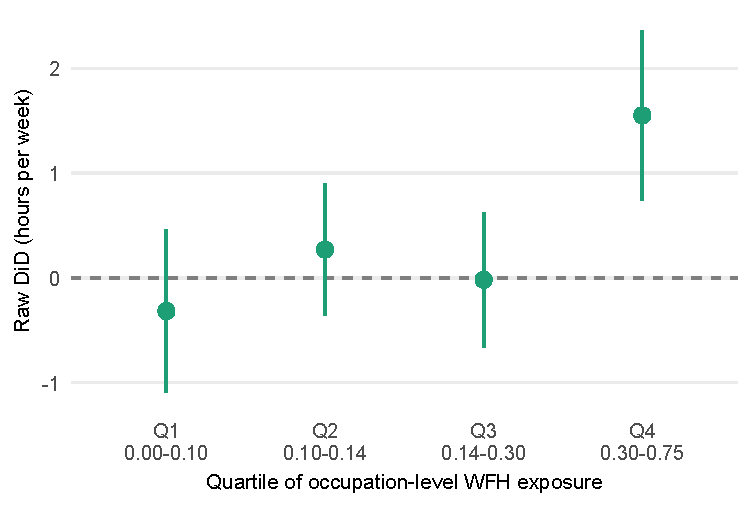
\includegraphics[width=0.59\textwidth]{../outputs/figures/hours_dose_response.pdf}
\caption{Unadjusted hours DiD within quartiles of calibrated WFH exposure}\label{fig:dose}
\begin{minipage}{0.82\textwidth}\small\setstretch{1}
\emph{Notes:} Respondents with observed usual hours and a matched occupation. Exposure cutoffs come from the pre-period; intervals use individual-clustered standard errors. The plotted 1.55 hours in the highest quartile is its DiD relative to the corresponding comparison women, not the difference between the highest and lowest quartiles. That latter raw contrast is approximately $1.55-(-0.32)=1.87$ hours.
\end{minipage}\end{figure}

\section{Empirical Strategy}\label{sec:strategy}
\subsection{Difference-in-differences and triple differences}
We begin with the change in the motherhood gap, using the common set of controls $X_{it}$:
\begin{equation}\label{eq:did}
Y_{it}=\beta_0+\beta_1\Mother_i+\beta_2\Post_t+\beta_3(\Mother_i\times\Post_t)+X'_{it}\gamma+\varepsilon_{it}.
\end{equation}
The coefficient $\beta_3$ is a differential change in hours among workers, or in employment in the full sample. It is not itself a measure of WFH exposure. To ask whether the differential change varies with occupational teleworkability $E_{j(i)}$, we estimate
\begin{equation}\label{eq:ddd}
\begin{split}
Y_{it}={}&\alpha+\delta_1\Mother_i+\delta_2\Post_t+\delta_3 E_{j(i)}
+\delta_4(\Mother_i\Post_t)\\
&+\delta_5(\Mother_i E_{j(i)})+\delta_6(\Post_t E_{j(i)})
+\delta_7(\Mother_i\Post_t E_{j(i)})+X'_{it}\gamma+\varepsilon_{it}.
\end{split}
\end{equation}
Here $\delta_7$ is the extra change in the mother/comparison gap per unit of exposure, while $\delta_4$ pertains to \emph{zero} exposure. The lower-order interactions permit an initial gap that depends on occupation exposure and a post-period exposure trend common to both groups. The relevant counterfactual is that the gap between mothers and comparison women at different exposure levels would have evolved similarly without the change in WFH opportunities \citep{olden2022}. This is not verified simply by showing that pre-period coefficients are statistically insignificant.

A linear slope compresses uneven effects into one number. Comparisons across exposure levels may have weights that are hard to interpret without further assumptions \citep{callaway2024}. We therefore estimate a saturated model with occupation-by-year, occupation-by-mother and mother-by-year effects, as well as a model with indicators for pre-period exposure quartiles. These models retain the triple-difference question while relaxing linear restrictions on lower-order patterns. The quartile model shows where the contrast arises.

\subsection{Inference and selection}\label{sec:inference}
Because respondents can appear in several survey waves, DiD errors are clustered by person. The occupational DDD is clustered by the 40 two-digit occupations; its analytic $p$-values use a $t$ distribution with 39 degrees of freedom. We also give a null-imposed wild cluster bootstrap with 9,999 draws \citep{roodman2019,fischer2021} and a test that permutes the 40 exposure scores across occupations 999 times \citep{phipson2010}. These procedures answer related but different inferential questions, and their disagreement is part of the evidence. Employment DDD inference clusters at the age-by-education-by-district cell level.

Hours are observed only for those who work in the reference week. Following the logic of \citet{lee2009}, we compare the observed hours selection rate among post-period mothers with a DiD-based counterfactual, trim the excess selected observations from opposite tails of their hours distribution, and re-estimate the interaction. For the DDD, trims occur within quartiles of the pre-period demographic-cell score. The resulting interval requires monotonic selection and the underlying comparison assumptions; we report a confidence interval for the identified set in the spirit of \citet{imbens2004}. It cannot address selection that violates monotonicity or differences in absence unrelated to excess selection.

\subsection{Diagnostics}
We estimate year-specific mother interactions relative to 2019, including an event study of the DDD. The occupational-score permutation test asks whether an equally large absolute $t$-statistic often arises when exposure labels are reassigned. We also test whether mothers' average occupation scores or probability of working in the highest exposure quartile change after 2021. Finally, we examine alternative scores, age balance, a sample without 2023, coding of hours as thresholds, child age and population group. The corresponding men's regression is a comparison across another exposed group, not a placebo with an expected zero effect.

\section{Results}\label{sec:results}
\subsection{Pre-period checks and the average hours change}\label{sec:did-results}
In the DiD event study, the 2017 and 2018 coefficients relative to 2019 jointly yield $F(2,63{,}198)=0.949$ ($p=0.387$). The main DiD estimate is 0.228 hours (SE 0.181; $N=251{,}857$). Its approximate 80\%-power minimum detectable effect is 0.51 hours, so the data offer some evidence against an average increase much larger than half an hour, conditional on the model. They cannot establish an exact zero. The event-study series shows its largest post-period estimate in 2023 (Figure~\ref{fig:event}).

\begin{figure}[htbp]\centering
\begin{minipage}[t]{0.48\textwidth}\centering
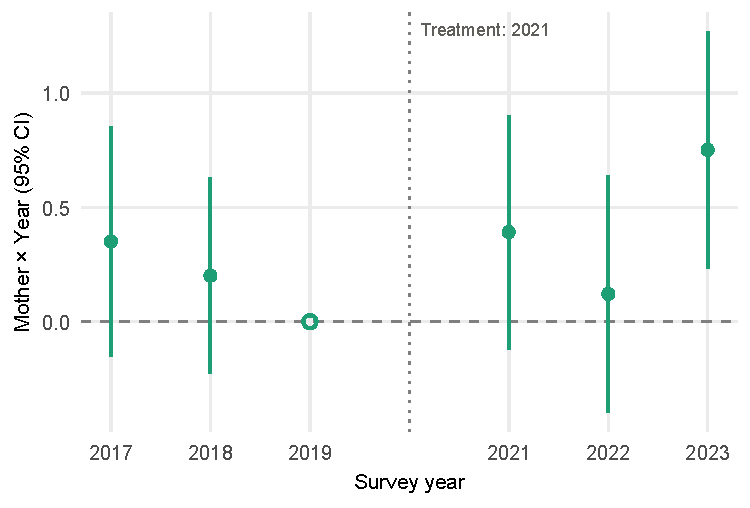
\includegraphics[width=\linewidth]{../outputs/figures/hours_event_study.pdf}\\{\small (a) Mother $\times$ survey year}
\end{minipage}\hfill
\begin{minipage}[t]{0.48\textwidth}\centering
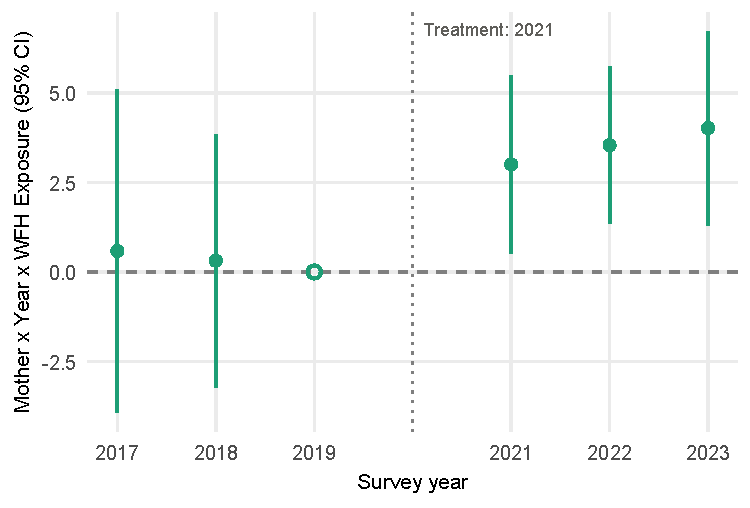
\includegraphics[width=\linewidth]{../outputs/figures/hours_ddd_event_study.pdf}\\{\small (b) Mother $\times$ year $\times$ exposure}
\end{minipage}
\caption{Event-study estimates for usual weekly hours; 2019 is the reference year}\label{fig:event}
\begin{minipage}{0.95\textwidth}\small\setstretch{1}\emph{Notes:} Panel (a) uses 251,857 observations and individual-clustered standard errors. Its pre-period joint test has $p=0.387$. Panel (b) uses 246,326 observations, the calibrated score and 40 occupation clusters; its pre-period joint Wald test has $p=0.960$. Bars show 95\% analytic confidence intervals. There is no 2020 extract; the 2019 marker denotes the omitted year.\end{minipage}
\end{figure}

\subsection{Exposure gradient in hours}\label{sec:ddd-results}
The main DDD estimate is 3.224 hours per unit of exposure (SE 1.022; $N=246{,}326$). Since a standard deviation of the score is 0.199, this is 0.640 hours per standard deviation. The difference in mean exposure between the top and bottom quartiles is $0.592-0.060=0.531$, implying $3.224\times0.531=1.71$ hours \emph{between} those quartiles. The corresponding raw contrast between their separate DiDs is 1.87 hours; the top quartile's DiD alone is 1.55 hours. These are three different quantities, and none should be described as an estimate of another. At zero exposure, the fitted motherhood change is $-0.539$ hours (SE 0.336), rather than the sample-average DiD.

Table~\ref{tab:hours} shows two functional-form checks. With occupation-by-year, occupation-by-mother and mother-by-year effects, the slope is 2.876 (SE 0.950). In a quartile model, the top-versus-bottom interaction is 1.844 hours (SE 0.595); the intermediate quartile interactions, 0.753 and 0.600, have confidence intervals that include zero. The association is therefore better described as concentrated in the most remote-capable occupations than as a uniform marginal effect across the full score. Only six of the 40 occupation categories fall in the highest quartile, a limitation for that contrast.

\begin{table}[htbp]\centering\begin{threeparttable}
\caption{Weekly-hours DiD and occupational-exposure DDD}\label{tab:hours}
\renewcommand{\baselinestretch}{1}\scriptsize\setlength{\tabcolsep}{3pt}
\begin{tabular}{lcccc}
\toprule
 & (1) DiD & (2) DDD & (3) DDD, saturated & (4) DDD, quartiles \\
\midrule
Mother $\times$ Post $\times$ WFH\_Exposure &  & $3.224$\sym{**} & $2.876$\sym{**} &  \\
 &  & $(1.022)$ & $(0.9495)$ &  \\
Mother $\times$ Post $\times$ Q2 (vs.\ Q1) &  &  &  & $0.7529$ \\
 &  &  &  & $(0.4827)$ \\
Mother $\times$ Post $\times$ Q3 (vs.\ Q1) &  &  &  & $0.5998$ \\
 &  &  &  & $(0.4847)$ \\
Mother $\times$ Post $\times$ Q4 (vs.\ Q1) &  &  &  & $1.844$\sym{**} \\
 &  &  &  & $(0.5946)$ \\
Mother $\times$ Post & $0.2280$ & $-0.5385$ &  & $-0.4720$ \\
 & $(0.1809)$ & $(0.3364)$ &  & $(0.3459)$ \\
Mother $\times$ WFH\_Exposure &  & $-1.295$ &  &  \\
 &  & $(1.053)$ &  &  \\
Post $\times$ WFH\_Exposure &  & $-0.5483$ &  &  \\
 &  & $(0.8102)$ &  &  \\
WFH\_Exposure &  & $1.128$ &  &  \\
 &  & $(3.912)$ &  &  \\
Mother & $-1.739$\sym{***} & $-1.449$\sym{***} &  & $-1.527$\sym{**} \\
 & $(0.1441)$ & $(0.3512)$ &  & $(0.4523)$ \\
Post & $-0.0570$ & $0.0535$ &  & $-0.1305$ \\
 & $(0.1481)$ & $(0.2732)$ &  & $(0.3666)$ \\
Constant & $32.35$\sym{***} & $32.12$\sym{***} &  & $31.58$\sym{***} \\
 & $(0.3182)$ & $(1.540)$ &  & $(2.051)$ \\
\midrule
MDE for triple interaction &  & $2.8640$ &  &  \\
SD of exposure, estimation sample &  & $0.1986$ &  &  \\
Triple interaction per SD of exposure &  & $0.640$ &  &  \\
Occupations in Q1 / Q2 / Q3 / Q4 &  &  &  & 16 / 7 / 11 / 6 \\
Fixed effects & None & None & Three sets & None \\
Observations & 251{,}857 & 246{,}326 & 246{,}324 & 246{,}326 \\
$R^2$ & 0.04049 & 0.04094 & 0.13512 & 0.04815 \\
Clustering & individual & occupation (40) & occupation (40) & occupation (40) \\
\bottomrule
\end{tabular}

\begin{tablenotes}\footnotesize\item All columns include age group, education, marital status, religion and district. Columns (2)--(4) require an occupation match. Column (3) includes three sets of lower-order fixed effects; column (4) uses pre-period exposure quartiles. DiD errors are clustered by person and DDD errors by occupation. The mother $\times$ post coefficient in columns (2) and (4) applies at zero exposure or in the omitted quartile, respectively. The table's MDE uses 39 degrees of freedom. \autonoteHours\end{tablenotes}
\end{threeparttable}\end{table}

\subsection{Pre-trends, selection and sorting}\label{sec:diagnostics-results}
The DDD event study finds small and imprecise pre-period interactions relative to 2019 (joint $F(2,39)=0.041$, $p=0.960$). Its post-period estimates are 3.011 in 2021, 3.545 in 2022 and 4.020 in 2023. The two pre-period standard errors, 2.237 and 1.745, are large beside the main estimate. Thus a lack of detectable pre-trends is reassuring only in a limited sense: the test cannot exclude economically relevant departures from parallel trends.

Trimming for excess post-period selection among mothers gives a lower DDD bound of 3.126 (SE 1.144) and an upper bound of 3.443 (SE 1.022). The reported 95\% interval for the identified set is $[1.021,5.324]$. These bounds depend on the selection assumptions and on the reference-week hours population. A separate sorting DiD using the occupation score as the outcome is 0.0013 (SE 0.0035); the change in the top-quartile share is 0.4 percentage points (SE 0.7). A DDD using the fixed demographic-cell index gives a positive but imprecise 0.139 hours per standard deviation (SE 0.159). These checks find no clear occupational shift by mothers, but the coarser cell index has less power to detect their own occupational teleworkability.

\begin{table}[htbp]\centering\begin{threeparttable}
\caption{Selection bounds for the occupational-exposure DDD}\label{tab:lee}
\renewcommand{\baselinestretch}{1}\small
\begin{tabular}{lccc}
\toprule
Bound & Coefficient & SE & 95\% CI \\
\midrule
Lower & $3.1255$ & $1.1440$ & $[0.8833,\ 5.3677]$ \\
Point (untrimmed) & $3.2319$ & $1.0538$ & $[1.1664,\ 5.2973]$ \\
Upper & $3.4434$ & $1.0220$ & $[1.4404,\ 5.4465]$ \\
\midrule
Imbens--Manski 95\% CI for the identified set &  &  & $[1.021,\ 5.324]$ \\
\bottomrule
\end{tabular}

\begin{tablenotes}\footnotesize\item Excess selection of post-period mothers is trimmed within quartiles of pre-period demographic-cell exposure. The untrimmed coefficient in this bound exercise differs slightly from the primary estimate because the estimation and trimming samples are not identical. The final row reports an interval for the identified set under the stated selection assumptions.\end{tablenotes}
\end{threeparttable}\end{table}

\subsection{Robustness and inference}\label{sec:robust}
The calibration choice is the most consequential specification choice. The fully pre-period external score gives 0.672 (SE 0.884), whereas the calibrated and realized measures give 3.224 (SE 1.022) and 5.195 (SE 2.363). Calibrating only on men's WFH responses yields 3.869 (SE 0.979). With the external score and separate mother/post terms for the ten replaced occupations, the external-score gradient becomes 2.339 (SE 1.352); dropping those ten occupations gives 4.309 (SE 1.192) across the remaining 30 clusters. These results weaken the claim that the calibrated estimate is an artifact of those occupations' own hours, but they cannot give a post-period calibrated index the status of a pre-treatment measure. A reader who regards the external score as uniquely credible should view the evidence as directional.

Age composition differs by motherhood status across exposure quartiles. Adding interactions between motherhood and age group gives 3.205 (SE 1.055); age-group reweighting gives 2.597 (SE 1.050). Omitting 2023 gives 2.979 (SE 1.170). Deleting one occupation at a time yields estimates between 2.415 and 3.580. Threshold outcomes indicate more movement across 35- and 40-hour cutoffs in higher-exposure occupations (0.096 and 0.107 per unit of exposure). Together these checks suggest that the association is not created by one occupation, 2023 alone or the choice of hour-bin medians. They do not solve the identifying assumptions.

Inference is sensitive to the small number of occupation clusters. The analytic test gives $p=0.0031$. The permutation test gives $p=0.0320$ and the null-imposed wild cluster bootstrap gives $p=0.0558$; the latter's 95\% confidence set includes zero. Accordingly, the strength of the statistical conclusion depends on the inference procedure. Table~\ref{tab:robust} reports the full sequence rather than selecting the most favorable result.

\begin{table}[htbp]\centering\begin{threeparttable}
\caption{Sensitivity of the hours triple interaction}\label{tab:robust}
\renewcommand{\baselinestretch}{1}\scriptsize\setlength{\tabcolsep}{2pt}
\begin{tabular}{lcccc}
\toprule
Specification & Coefficient & SE & $p$ & $N$ \\
\midrule
\multicolumn{5}{l}{\emph{Exposure measure}} \\
\quad Calibrated (primary) & $3.224$\sym{**} & $1.022$ & $0.0031$ & 246{,}326 \\
\quad External (Dingel--Neiman) & $0.6720$ & $0.8838$ & $0.4517$ & 246{,}326 \\
\quad Realized (2021 anchor) & $5.195$\sym{*} & $2.363$ & $0.0346$ & 246{,}037 \\
\multicolumn{5}{l}{\emph{Age balance}} \\
\quad Age-interacted ($+\,\Mother \times$ age group) & $3.205$\sym{**} & $1.055$ & $0.0042$ & 246{,}326 \\
\quad Reweighted (pre-period age-group raking) & $2.597$\sym{*} & $1.050$ & $0.0178$ & 242{,}552 \\
\multicolumn{5}{l}{\emph{Sample}} \\
\quad Unswapped occupations only (30 of 40) & $4.309$\sym{**} & $1.192$ & $0.0011$ & 132{,}046 \\
\quad Excluding survey year 2023 & $2.979$\sym{*} & $1.170$ & $0.0151$ & 208{,}833 \\
\multicolumn{5}{l}{\emph{Outcome coding}} \\
\quad Irregular-hours codes dropped, not imputed & $3.056$\sym{**} & $1.059$ & $0.0064$ & 232{,}785 \\
\quad Full-time indicator ($\geq 35$ hours) & $0.0964$\sym{**} & $0.0291$ & $0.0020$ & 246{,}326 \\
\quad Long-hours indicator ($\geq 40$ hours) & $0.1073$\sym{**} & $0.0380$ & $0.0075$ & 246{,}326 \\
\multicolumn{5}{l}{\emph{Inference on the primary estimate}} \\
\quad Two-way clustering (individual, occupation) & $3.224$\sym{**} & $1.022$ & $0.0031$ & 246{,}326 \\
\quad Wild cluster bootstrap ($B = 9{,}999$) & $3.224$ & $1.022$ & $0.0558$ & 246{,}326 \\
\quad Permutation test (999 reassignments) & $3.224$ &  & $0.0320$ & 246{,}326 \\
\bottomrule
\end{tabular}

\begin{tablenotes}\footnotesize\item Unless indicated, rows re-estimate the mother $\times$ post $\times$ exposure coefficient with standard controls and occupation clustering. The external-score model with replaced-occupation interactions contains both reported coefficients. The pre-period cell-score result is scaled by that index's SD and uses cell clustering. Threshold outcomes are linear probability models. Permutation and bootstrap rows report their own $p$-values rather than analytic $t$-test values.\end{tablenotes}
\end{threeparttable}\end{table}

\subsection{Child age, population groups and fathers}\label{sec:heterogeneity}
The exposure slope is largest when the youngest child is under five: 3.656 (SE 1.079), compared with 3.211 (SE 1.311), 2.741 (SE 1.525) and 1.862 (SE 0.935) in successive child-age bands. The same comparison women enter each regression; overlapping intervals preclude a firm claim that the child-age effects differ. For Jewish women the slope is 2.847 (SE 0.913), and for Arab women it is 5.507 (SE 2.674). Although the point estimates differ, a formal comparison does not distinguish them ($p=0.35$), so the smaller subgroup does not establish a stronger effect.

For men, defining fatherhood analogously, the corresponding DDD estimate is $-1.762$ (SE 1.015). The difference between women's and men's slopes is statistically distinguishable in the reported two-sample comparison ($z=3.461$, $p=0.0005$). This rules against a simple exposure-related hours increase common to both sexes. It does not demonstrate a within-household transfer of care: individual mothers and fathers are not linked, and the male coefficient itself is imprecise.

\begin{table}[htbp]\centering\begin{threeparttable}
\caption{Hours estimates by age of the youngest child}\label{tab:childage}
\renewcommand{\baselinestretch}{1}\footnotesize\setlength{\tabcolsep}{3pt}
\begin{tabular}{lcccccc}
\toprule
 & \multicolumn{3}{c}{DiD: $\Mother \times \Post$} & \multicolumn{3}{c}{DDD: $\Mother \times \Post \times \WFH$} \\
\cmidrule(lr){2-4}\cmidrule(lr){5-7}
Sample of mothers & Coef. & SE & $N$ & Coef. & SE & $N$ \\
\midrule
All mothers (Table~\ref{tab:hours}) & $0.2280$ & $0.1809$ & 251{,}857 & $3.224$\sym{**} & $1.022$ & 246{,}326 \\
\midrule
Youngest child aged 0--4 & $0.1267$ & $0.2111$ & 158{,}424 & $3.656$\sym{**} & $1.079$ & 154{,}499 \\
Youngest child aged 5--9 & $0.1621$ & $0.2533$ & 130{,}782 & $3.211$\sym{*} & $1.311$ & 127{,}419 \\
Youngest child aged 10--14 & $0.1593$ & $0.2780$ & 123{,}280 & $2.741$\sym{\cdot} & $1.525$ & 120{,}084 \\
Youngest child aged 15--17 & $0.5613$ & $0.3483$ & 107{,}061 & $1.862$\sym{\cdot} & $0.9354$ & 104{,}079 \\
\bottomrule
\end{tabular}

\begin{tablenotes}\footnotesize\item Each child-age sample compares mothers in the indicated group with the same comparison population. DiD errors cluster by individual, DDD errors by occupation. Rows overlap in their comparison observations. \autonoteChildAge\end{tablenotes}
\end{threeparttable}\end{table}

\begin{table}[htbp]\centering\begin{threeparttable}
\caption{Hours estimates by population group and for fathers}\label{tab:subgroup}
\renewcommand{\baselinestretch}{1}\footnotesize\setlength{\tabcolsep}{3pt}
\begin{tabular}{lcccccc}
\toprule
 & \multicolumn{3}{c}{DiD: $\Mother \times \Post$} & \multicolumn{3}{c}{DDD: $\Mother \times \Post \times \WFH$} \\
\cmidrule(lr){2-4}\cmidrule(lr){5-7}
Subgroup & Coef. & SE & $N$ & Coef. & SE & $N$ \\
\midrule
All women (primary) & $0.2280$ & $0.1809$ & 251{,}857 & $3.224$\sym{**} & $1.022$ & 246{,}326 \\
Jewish women & $0.3021$ & $0.2027$ & 214{,}449 & $2.847$\sym{**} & $0.9125$ & 209{,}727 \\
Arab women & $-0.0724$ & $0.4785$ & 24{,}975 & $5.507$\sym{*} & $2.674$ & 24{,}307 \\
Men (fathers vs.\ childless) & $-0.4002$\sym{*} & $0.1883$ & 261{,}543 & $-1.762$\sym{\cdot} & $1.015$ & 251{,}779 \\
\midrule
95\% CI, Jewish & \multicolumn{3}{c}{$[-0.0952,\ 0.6994]$} & \multicolumn{3}{c}{$[1.0579,\ 4.6351]$} \\
95\% CI, Arab & \multicolumn{3}{c}{$[-1.0103,\ 0.8656]$} & \multicolumn{3}{c}{$[0.2657,\ 10.7481]$} \\
Jewish vs.\ Arab, $z$ ($p$) & \multicolumn{3}{c}{$0.720$ (0.471)} & \multicolumn{3}{c}{$-0.942$ (0.346)} \\
Women vs.\ men, $z$ ($p$) & \multicolumn{3}{c}{$2.406$ (0.016)} & \multicolumn{3}{c}{$3.461$ (0.001)} \\
\bottomrule
\end{tabular}

\begin{tablenotes}\footnotesize\item Women are compared by motherhood status; for men the comparison is between fathers and men without a child under 17 in the household. DiD standard errors cluster by person and DDD standard errors by occupation. The subgroup point estimates are not formal evidence of heterogeneous effects; the comparison-test rows give the relevant tests. \autonoteSubgroup\end{tablenotes}
\end{threeparttable}\end{table}

\subsection{Employment as a secondary outcome}\label{sec:employment}
The employment DiD is $-0.0053$ (SE 0.0052): no detectable average post-period change in mothers' employment relative to other women's. The employment DDD, using the pre-period cell score, is $-0.0257$ (SE 0.0725). That interaction is much less informative. Its minimum detectable effect is 1.43 percentage points per SD of the cell score, larger than the effect scale suggested by \citet{harrington2025}. Consequently, the employment DDD cannot adjudicate whether WFH changed the employment penalty. The two outcomes have different samples and exposure definitions, so their coefficients should not be compared directly.

\begin{table}[htbp]\centering\begin{threeparttable}
\caption{Employment outcomes as a secondary analysis}\label{tab:employment}
\renewcommand{\baselinestretch}{1}\small\setlength{\tabcolsep}{5pt}
\begin{tabular}{lcc}
\toprule
 & (1) DiD & (2) DDD, cell-based exposure \\
\midrule
Mother $\times$ Post $\times$ WFH\_Exposure &  & $-0.0257$ \\
 &  & $(0.0725)$ \\
Mother $\times$ Post & $-0.0053$ & $0.0065$ \\
 & $(0.0052)$ & $(0.0168)$ \\
Mother $\times$ WFH\_Exposure &  & $-0.1404$\sym{\cdot} \\
 &  & $(0.0803)$ \\
Post $\times$ WFH\_Exposure &  & $-0.1555$\sym{**} \\
 &  & $(0.0566)$ \\
WFH\_Exposure &  & $0.0131$ \\
 &  & $(0.0565)$ \\
Mother & $-0.0034$ &  \\
 & $(0.0041)$ &  \\
Post & $0.0153$\sym{***} &  \\
 & $(0.0043)$ &  \\
Constant & $0.4926$\sym{***} &  \\
 & $(0.0085)$ &  \\
\midrule
MDE ($\alpha=0.05$, power $0.80$), per unit &  & $0.2031$ \\
MDE per SD of exposure &  & $0.0143$ \\
\quad as \% of baseline employment rate &  & 1.85\% \\
\midrule
Observations & 364{,}784 & 355{,}984 \\
$R^2$ & 0.227 & 0.221 \\
Clustering & individual & demographic cell ($\approx 210$) \\
\bottomrule
\end{tabular}

\begin{tablenotes}\footnotesize\item Binary employment outcome for women aged 25--59. The DDD uses a pre-period demographic-cell index because occupation is unavailable for the non-employed; its scale and sample differ from the hours DDD. DiD standard errors cluster by individual; DDD standard errors cluster by demographic cell. All outcome estimates are unweighted.\end{tablenotes}
\end{threeparttable}\end{table}

\section{Discussion}\label{sec:discussion}
The evidence is consistent with a selective rather than a broad hours response. Mothers' relative hours show little average change, while the largest response appears in occupations with high WFH exposure. For a worker at the mean exposure of the highest quartile (about 0.592), the fitted change relative to comparison women is $-0.539+3.224(0.592)\approx1.37$ hours. This quantity differs from the 1.71-hour \emph{between-quartile} fitted contrast and from the 1.55-hour raw DiD \emph{within} the highest quartile. Keeping those quantities separate prevents the pattern from sounding more precise than it is.

One plausible mechanism is that WFH relaxes a scheduling constraint in jobs where work can be done elsewhere, particularly for mothers of younger children. Saved travel time could be reassigned to paid work, consistent with evidence that WFH reduces commuting time \citep{aksoy2023}. Yet the design measures occupational exposure and hours, not individual time use or exogenous WFH assignment. Changes in employers' demands for mothers, reporting practices or occupation-specific shocks that interact with parenthood could also generate the observed gradient. The saturated specification absorbs shocks common to mothers and comparison women within an occupation and year, and the fathers' pattern weighs against a shock shared by all workers, but neither rules out a mother-specific shock.

The distinction from US evidence is also substantive. \citet{harrington2025} report employment and income changes; we observe hours but no income amount. A conditional-hours association among Israeli working mothers cannot by itself establish an earnings effect or a general increase in participation. The potential policy implication is narrower: flexibility may alter paid hours for mothers already in remote-capable jobs, a group whose access to those jobs is itself unequal. The size of any population-wide gain remains unknown without representative weighting and a credible estimate of the employment margin.

\section{Limitations}\label{sec:limitations}
\paragraph{Identification and measurement.} A statistically quiet pre-period event study cannot prove parallel trends with 40 occupation clusters. The main exposure index incorporates 2022--2023 information; the wholly external alternative has a much smaller, insignificant slope. Two-digit codes average over workplace and within-occupation differences, while Israel's institutional practice can diverge from an international task classification. Neither the calibration checks nor the sorting tests make occupation exposure as good as randomly assigned.

\paragraph{Conditional hours and selection.} The outcome is usual hours for women who worked in the reference week. Approximately 10\% of employed observations are excluded, and the probability of absence can vary with both exposure and motherhood. Lee-style trimming addresses a specified excess-selection pattern under monotonicity. Other forms of selection into employment, reference-week work and occupation remain possible. Hours are bin medians; threshold specifications corroborate a pattern around full-time cutoffs but do not recover exact hours worked.

\paragraph{Period, comparison group and inference.} The last quarter of 2023 coincided with the start of the October 2023 war, which could change hours and caregiving in ways our regressions do not isolate. Excluding 2023 leaves a positive estimate, but early 2021 includes a lockdown. The comparison group can contain mothers of older children or women who become mothers during the sample window. Estimates are unweighted and conditional on observed covariates. The analytic, score-permutation and bootstrap tests give different levels of confidence; score permutation also assumes that occupations' exposure labels are exchangeable under its null. Reporting only the smallest $p$-value would obscure these limitations.

\section{Conclusion}\label{sec:conclusion}
Using Israeli survey data, we ask whether the expansion of remote work coincided with a change in the motherhood penalty in usual weekly hours. The average change among women observed working is small, whereas the post-2021 change in the mother/comparison gap increases with an occupation's calibrated WFH exposure. The strongest contrast is at the top of the exposure distribution and among mothers with younger children. Those patterns are consistent with greater scheduling flexibility helping some already employed mothers supply more paid hours.

The result is conditional and does not establish a universal benefit from remote work. The exposure score partly uses post-period WFH information; the wholly external score yields a weaker result, pre-trend tests have limited power, and inference varies with the procedure. Employment is an important separate margin, but its exposure interaction is too imprecise here to settle the question. The data also contain no earnings amount. Stronger evidence would link hours with earnings and household time use, measure exposure before treatment in the Israeli setting, and estimate women's and men's responses together on a design that better separates access to WFH from occupation choice.

\begin{spacing}{1}
\bibliographystyle{apalike}
\bibliography{references}
\end{spacing}
\end{document}
